\chapter{Введение}
Цель данной работы заключается в реализации метрики, основанной на прокладывании маршрутов на
картах OpenStreetMap, а также внедрение этой метрики в работу алгоритмов K-Means и Mean Shift.
В данной работе для реализации прокладывания маршрутов на карте используется фреймворк
Project OSRM.

Фреймворк OSRM (\emph{Open Source Routing Machine}) является свободным и работает с картами
сообщества OpenStreetMap. Фреймворк широко используется для написания приложений для различных
навигаторов, поскольку позволяет не только находить кратчайший маршрут между двумя точками, но и
выдавать инструкции по передвижению.

Алгоритм Mean Shift (среднего сдвига) является центроидным алгоритмом кластеризации, зачастую
применяется в задачах низкоуровневого компьютерного зрения вследствие легкости и эффективности.
Алгоритм среднего сдвига основан на ядре оценки плотности.

Алгоритм K-Means (K-средних) является центроидным алгоритмом кластеризации. Широко применяется в
задачах классификации и кластеризации, а также для задач машинного зрения и глубокого обучения.
Алгоритм стремится минимизировать суммарное квадратичное отклонение точек кластеров от центров этих
кластеров. Проблемой алгоритма является то, что результат кластеризации сильно зависит от выбора
начальных центров кластеров, а также то, что число кластеров необходимо знать заранее.

Scikit-learn~-- открытая python-библиотека машинного обучения. В ней содержатся различные алгоритмы
классификации, кластеризации и регрессионного анализа.

\newpage

\chapter{Алгоритм Mean Shift}
\section{Суть алгоритма}
Алгоритм кластеризации Mean Shift направлен на обнаружение сгустков плотности среди заданного
набора образцов. Он является центроидным, то есть работает посредством обновления положения центров
плотности. На каждой итерации алгоритма высчитывается среднее взвешенное значение плотности
образцов в заданной области с использованием особой функции, называемой ядром~\eqref{eq:1}:
\begin{equation}
    m(x) = \frac{\sum_{x_i \in N(x)} K(x_i - x)x_i}{\sum_{x_i \in N(x)} K(x_i - x)},
    \label{eq:1}
\end{equation}
где \( m(x) \)~-- среднее взвешенное значение плотности в заданной области, \( N(x) \)~--
соседние к \( x \) образцы, причем для них \( K(x) \ne 0 \), \( K(x_i - x) \)~-- ядро.

В ядре содержится единственный параметр, используемый в данном ал\-го\-рит\-ме~\eqref{eq:2}:
\begin{equation}
    K(x_i - x) = k\left( \frac{\|x_i - x\|^2}{h^2} \right).
    \label{eq:2}
\end{equation}
Параметр \( h \), называемый <<пропускной способностью>> (\emph{bandwidth}), в данном
ал\-го\-рит\-ме регулирует размер области, в которой ищутся соседние образцы и рассчитывается
среднее значение плотности. Функция \( k \) здесь -- профиль ядра.

Обычно в качестве ядра используют гауссианы~\eqref{eq:3}:
\begin{equation}
    K(x_i - x) = e^{-c\|x_i - x\|^2}.
    \label{eq:3}
\end{equation}

После расчета \( m(x) \) алгоритм заменяет положение центроидов \( x \) на рас\-счи\-тан\-ные
\( m(x) \), и переходит к следующей итерации.

В период пост-обработки центроиды фильтруются, отбрасываются дуб\-ли\-ка\-ты и близлежащие
центроиды, после чего формируется окончательный набор центроидов.~\cite{vorontsov, ms, ms2}

Сильные стороны алгоритма:
\begin{itemize}
    \item весь процесс кластеризации зависит только от одного параметра \( h \), имеющего реальный
        физический смысл;
    \item нет зависимости от размерности пространства и конкретной метрики расстояний;
    \item не предполагает конкретных форм кластеров.
\end{itemize}

Слабые стороны алгоритма:
\begin{itemize}
    \item выбор параметра \( h \) весьма нетривиален, зачастую требует адаптивной подстройки во
        время работы алгоритма; а неправильный выбор этого параметра может приводить к схопыванию
        кластеров или генерации дополнительных кластеров, в которых плотность образцов невелика;
    \item алгоритм является очень ресурсоемким: в общем он требует \( O(kN^2) \) операций, где
        \( N \)~-- число образцов, \( k \)~-- среднее количество итераций на один образец.
\end{itemize}

На рисунках~\ref{pic:1} и~\ref{pic:2} для сравнения приведены соответственно результаты
кластеризации одной и той же выборки алгоритмами K-Means и Mean Shift.

\begin{figure}[hp!]
    \center
    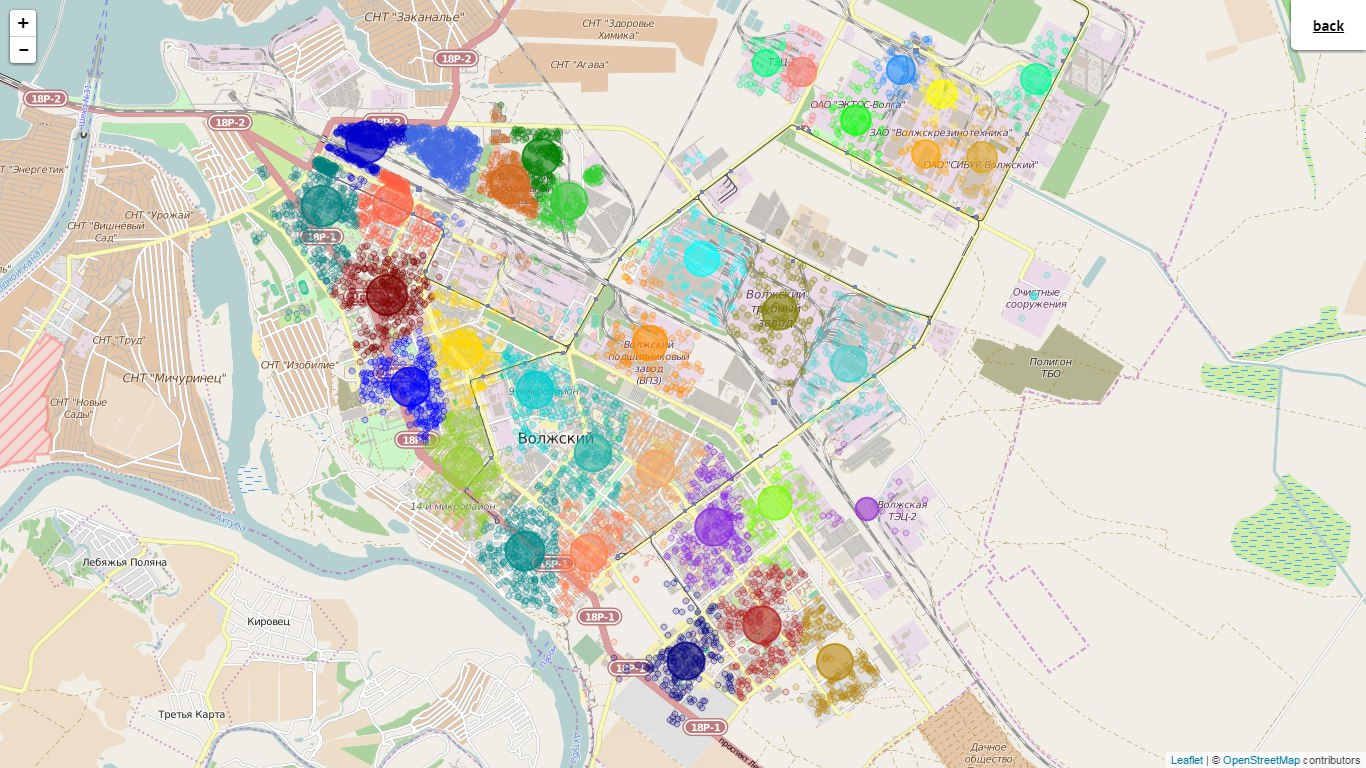
\includegraphics[width=.8\textwidth]{km}\\
    \parbox{.8\textwidth}{\centering
        \caption{Результаты кластеризации алгоритмом K-Means} \label{pic:1}}\\
    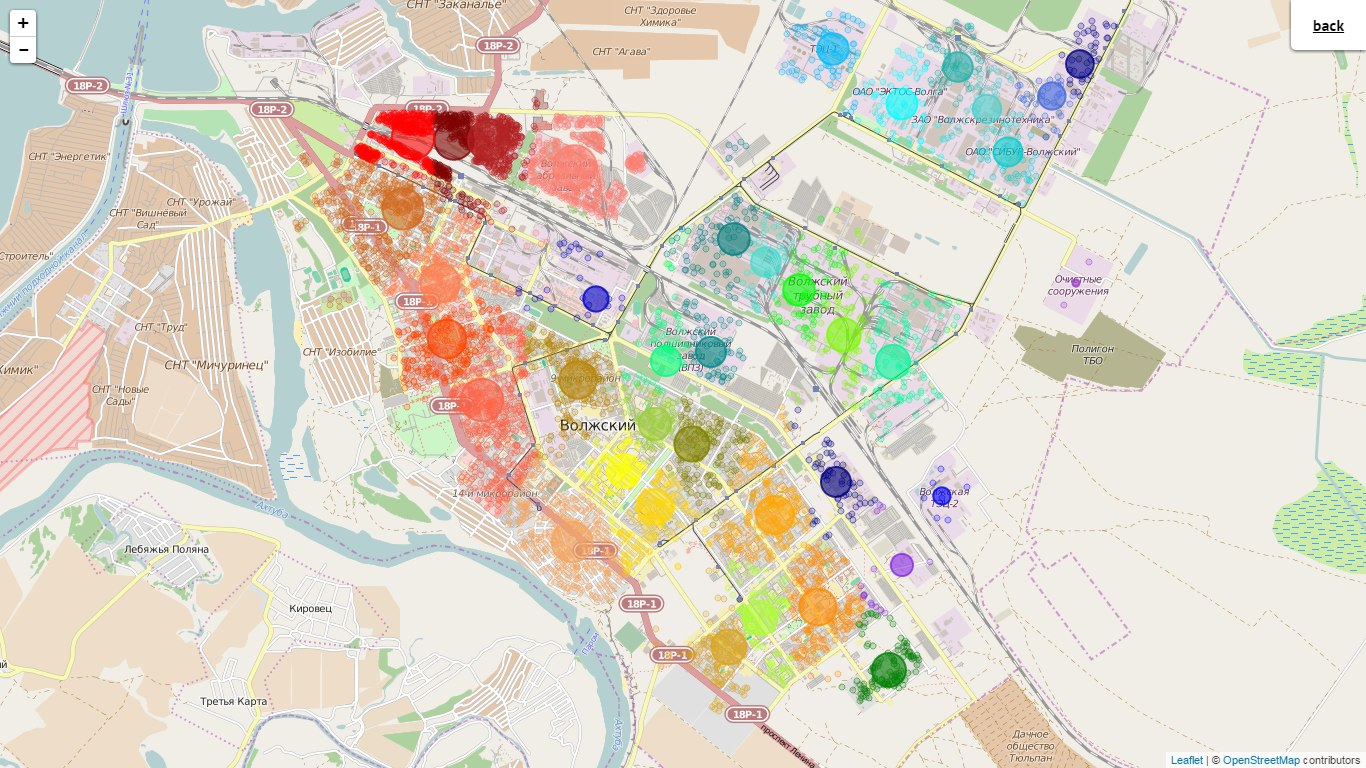
\includegraphics[width=.8\textwidth]{mn}\\
    \parbox{.8\textwidth}{\centering
        \caption{Результаты кластеризации алгоритмом Mean Shift} \label{pic:2}}
\end{figure}

\section{Реализация}
Алгоритм Mean Shift был реализован на языке программирования Python с использованием
библиотек numpy и scikit-learn~\cite{scikit} Также при написании ис\-поль\-зуют\-ся ранее написанные модули
ClusteringMachine~(прил.~\ref{sec:cm}) и\\ DataCollector~(прил.~\ref{sec:dc}).
Реали\-за\-ция пред\-став\-ляет собой подключаемый модуль~(прил.~\ref{sec:mss}),
который можно запускать и как обыч\-ный Python-скрипт.

\newpage

\chapter{Построение маршрутов}
Для нахождения расстояния между двумя точками с помощью построения маршрута между ними используется
фреймворк Project-OSRM ({\small\url{http://project-osrm.org}}).

\section{Установка и настройка Project-OSRM}
Подробная информация об установке и настройке OSRM на различные ОС находится в документации
проекта~\cite{osrm}.

\textbf{Для ОС Fedora.}
Произведите установку git, cython, cmake и gcc-c++:
\begin{lstlisting}
$ sudo yum install git cython cmake gcc-c++
\end{lstlisting}

Установите необходимые зависимости:
\begin{lstlisting}
$ sudo yum install libxml2-devel boost-devel boost-regex bzip2-devel \
  libzip-devel stxxl-devel protobuf-devel protobuf-lite protobuf-lite-devel \
  lua.x86_64 lua-devel.x86_64 luajit.x86_64 luajit-devel.x86_64 \
  luabind.x86_64 luabind-devel.x86_64 expat expat-devel tbb tbb-devel
\end{lstlisting}

Скачайте и установите библиотеку для чтения и записи PBF файлов:
\begin{lstlisting}
$ git clone https://github.com/scrosby/OSM-binary.git
$ cd OSM-binary
$ cmake .
$ sudo make install
\end{lstlisting}

Скачайте и установите Project-OSRM:
\begin{lstlisting}
$ git clone https://github.com/DennisOSRM/Project-OSRM.git
$ mkdir –p Project-OSRM/build
$ cd Project-OSRM/build
$ cmake ..
$ make
$ sudo make install
\end{lstlisting}

Скачайте и установите серверную часть Project-OSRM:
\begin{lstlisting}
$ git clone https://github.com/Project-OSRM/osrm-backend.git
$ cd osrm-backend
$ mkdir -p build
$ cd build
$ cmake ..
$ make
\end{lstlisting}

Не выходя из директории \emph{build} сделайте символическую ссылку на скоростной профиль и
директорию с библиотеками для скоростных профилей. Стандартным скоростным профилем является
профиль автомобиля:
\begin{lstlisting}
$ ln -s ../profiles/car.lua profile.lua
$ ln -s ../profiles/lib/
\end{lstlisting}

Распакуйте необходимую OpenStreetMap-карту:
\begin{lstlisting}
$ osrm-extract map.osm
\end{lstlisting}

Результатом выполнения команды будет файл \emph{map.osrm}. Выполните обработку данных карты:
\begin{lstlisting}
$ osrm-prepare map.osrm
\end{lstlisting}
Результатом будет набор из 9 файлов, каждый из которых содержит определенную часть загруженной
карты.

Запускаем сервер Project-OSRM:
\begin{lstlisting}
$ osrm-routed map.osrm
\end{lstlisting}

\section{Реализация метрики}
Реализуемая метрика была названа \emph{route}~(прил.~\ref{sec:route}). Модуль содержит класс
\emph{route}, в котором есть три функции: \emph{start}, \emph{stop} и \emph{route\_distance}.

Первая функция запускает процесс \emph{osrm-routed} с нужным файлом карты.

Вторая функция останавливает запущенную OSRM машину.

Третья функция возвращает дистанцию между двумя точками, пе\-ре\-дан\-ных ей в качестве параметров.

Было реализовано локальное хранение данных о построенных маршрутах в виде текстового файла,
подгружаемого при старте OSRM машины и перезаписываемого при ее остановке. Это позволяет сократить
время на кластеризацию, поскольку при повторении запроса происходит извлечения значения расстояния
из памяти без повторного построения маршрута.

\newpage

\chapter{Внедрение метрики}
\section{Внедрение метрики в алгоритм K-Means}
Для внедрения метрики в модуль с алгоритмом K-Means необходимо импортировать написанный
мо\-дуль метрики; добавить поле \emph{route\_} классу, который отвечает за расчет расстояний;
прописать этот расчет и прописать запуск и остановку OSRM машины~(прил.~\ref{sec:km}).

\section{Внедрение метрики в алгоритм Mean Shift}
Для внедрения метрики в модуль с алгоритмом Mean Shift также необходимо импортировать написанный
мо\-дуль метрики; добавить поле \emph{route\_} классу, который отвечает за расчет расстояний;
прописать этот расчет и прописать запуск и остановку OSRM машины:\\
\ldots
\lstinputlisting[language=Python,firstline=7,lastline=9]{meanshift.py}
\ldots
\lstinputlisting[language=Python,firstline=29,lastline=33]{meanshift.py}
\ldots
\lstinputlisting[language=Python,firstline=44,lastline=51]{meanshift.py}
\ldots

Теперь при запуске кластеризации с помощью модуля Mean Shift будет производится запуск и остановка
OSRM машины, однако будет использоваться прежняя метрика~-- декартова, поскольку сам алгоритм
находится внутри подключаемой библиотеки Scikit-learn.

Скачиваем библиотеку Scikit-learn:
\begin{lstlisting}
$ git clone https://github.com/scikit-learn/scikit-learn.git
\end{lstlisting}

Копируем в директорию модуль метрики, переходим в директорию~\emph{sklearn}:
\begin{lstlisting}
$ cp route.py scikit-learn/sklearn/
$ cd scikit-learn/sklearn/
\end{lstlisting}

Алгоритм Mean Shift находится в файле \emph{cluster/mean\_shift\_.py}.
Добавляем выбор метрики: параметром прописываем \emph{metric = 'route'}.

Теперь нужно написать саму метрику, которую алгоритм мог бы выбрать.
В файле \emph{metrics/pairwise.py} добавляем новую метрику \emph{`route`} и прописываем в
списках доступных метрик новую.

Для того, чтобы алгоритм поиска соседей также мог пользоваться метрикой, прописываем метрику в
файл \emph{neighbors/dist\_metric.pyx}. Для сохранения сделанных изменений в этом файле
необходимо скомпилировать c-библиотеку:
\begin{lstlisting}
$ cd neighbors
$ cython dist_metric.pyx
\end{lstlisting}

Добавляем прописанную метрику в список доступных метрик в файле с алгоритмом поиска соседей
\emph{neighbors/ball\_tree.pyx}.

Если при первом запуске начальные центры кластеров становятся в точку с координатами
\texttt{(0, 0)}, то в файле с алгоритмом Mean Shift\\ (\emph{cluster/mean\_shift\_.py}) необходимо
изменить строчку:
\begin{lstlisting}[language=Python]
binned_point = np.round(point / bin_size)
\end{lstlisting}

В этом месте для упрощения расчетов координаты делятся на размер рассматриваемой области
и округляются. Для задачи кластеризации географических координат размер области на 1-2 порядка
превышает значения координат. Поэтому необходимо оставить определенное количество цифр после
запятой:
\begin{lstlisting}[language=Python]
binned_point = np.round(point / bin_size, decimals = 5)
\end{lstlisting}

Собираем и устанавливаем измененную библиотеку:
\begin{lstlisting}
$ cd ..
$ python setup.sh build
$ sudo python setup.sh install
\end{lstlisting}

Теперь вместо библиотеки \emph{scikit-learn} установлена ее измененная версия, в которую
добавлена новая метрика; таким образом, модуль с алгоритмом Mean Shift теперь также поддерживает
метрику \emph{route}.

\newpage

\chapter{Выводы}
При использовании реализованной метрики заметно повысилась точность кластеризации географических
данных~-- учитывается ландшафт местности и естественные препятствия: железные дороги, реки,
овраги и балки. Однако, существенно понизилась скорость выполнения кластеризации:
на один запрос расчета дистанции между двумя точками требуется примерно 10~мсек.
Таким образом, на то, чтобы рассчитать только расстояния между всеми точками тестовой выборки
(6000 точек) необходимо потратить:
\[
    t = \frac{6000!}{2 * 5998!} \cdot 10 = 179970000\textrm{ мсек} \approx 50\textrm{ ч}.
\]

Использование локального хранения рассчитанных значений ускоряет процесс: на полную кластеризацию
200 точек (от 25 до 50 итераций) алгоритм K-Means тратит от 60 до 180 секунд, тогда как только на
одну итерацию (при 40 кластерах) должно уходить около 80 секунд.

На рисунках~\ref{pic:3}~--~\ref{pic:5} приведены результаты кластеризации 200 точек алгоритмами
K-Means и Mean Shift.

\begin{figure}[hp!]
    \center
    \vspace{-1cm}
    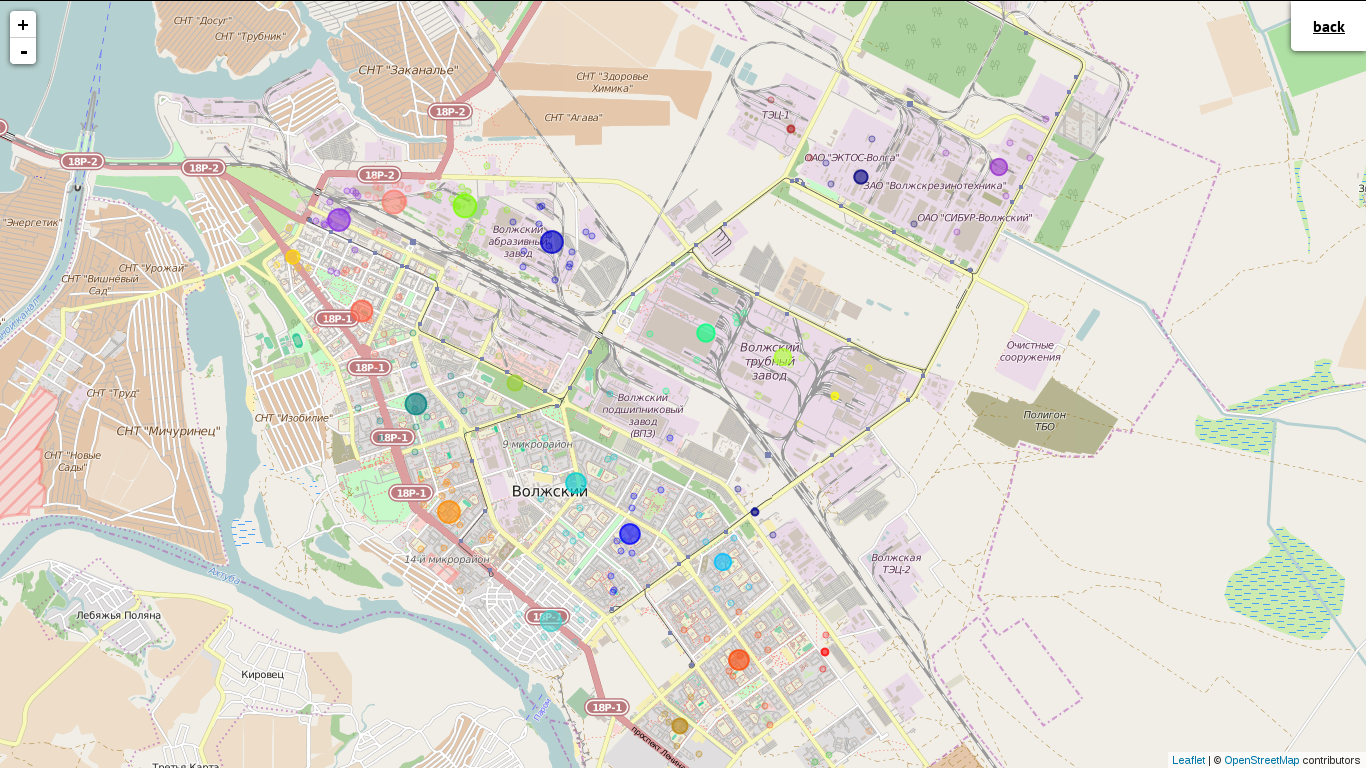
\includegraphics[width=.8\textwidth]{km_eu}\\
    \parbox{.8\textwidth}{\centering
        \caption{Результаты кластеризации алгоритмом K-Means с евклидовой
            метрикой} \label{pic:3}}\\
    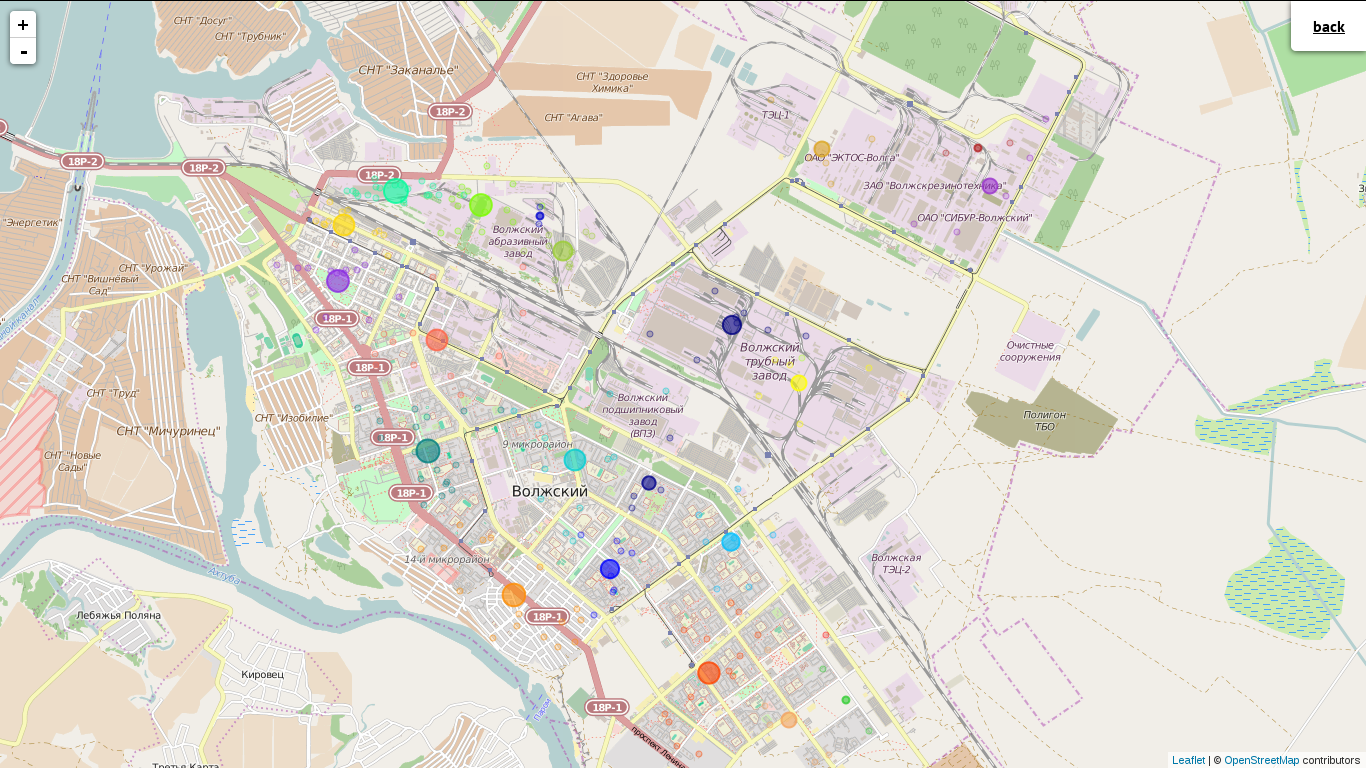
\includegraphics[width=.8\textwidth]{km_ro}\\
    \parbox{.8\textwidth}{\centering
        \caption{Результаты кластеризации алгоритмом K-Means с метрикой route} \label{pic:4}}\\
    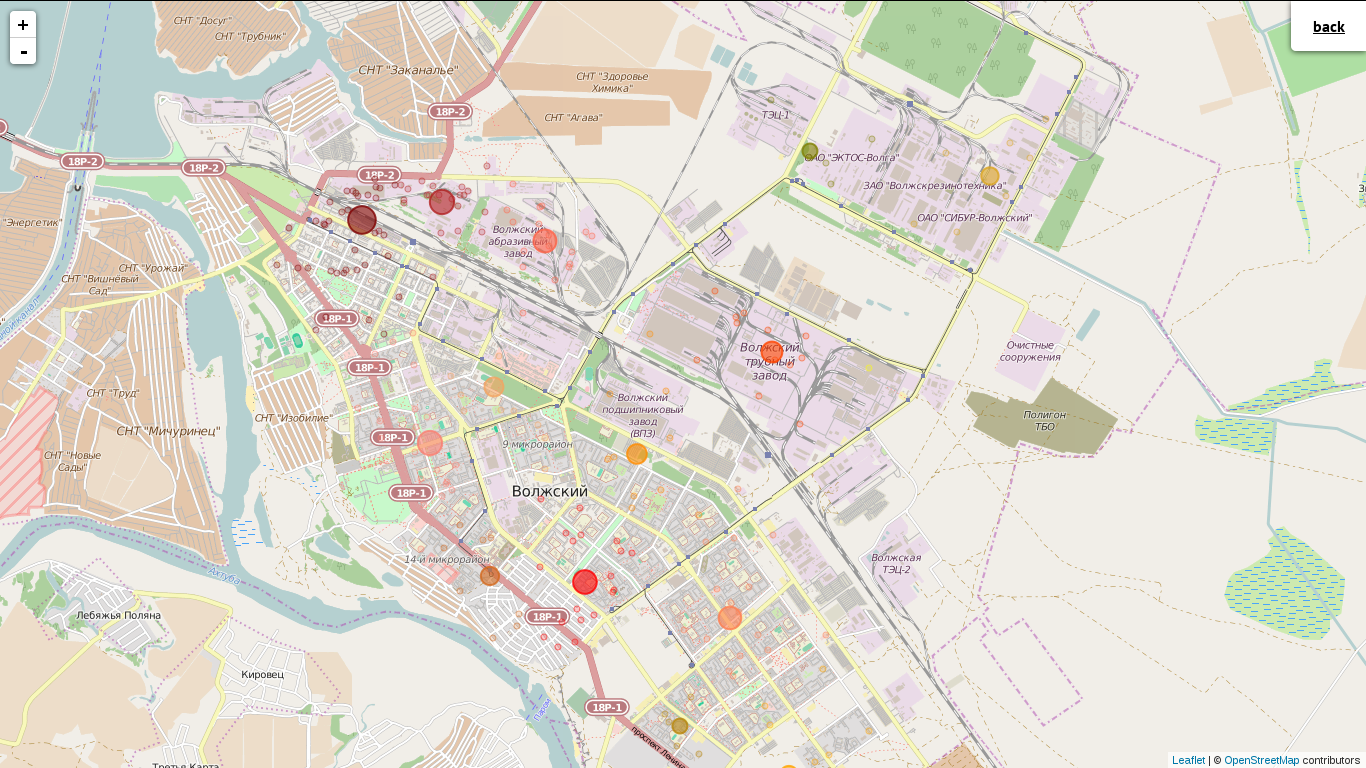
\includegraphics[width=.8\textwidth]{mn_eu}\\
    \parbox{.8\textwidth}{\centering
        \caption{Результаты кластеризации алгоритмом Mean Shift с евклидовой
            метрикой} \label{pic:5}}
\end{figure}

\newpage

\chapter{Результаты}
В результате выполнения можно заключить следующее:
\begin{enumerate}\itemsep-.5ex
    \item Проведен анализ различных источников информации по теме работы.
    \item Произведена реализация модуля кластеризации алгоритмом Mean Shift.
    \item Произведена установка фреймворка Project OSRM.
    \item Произведена реализация модуля метрики, основанной на построении маршрутов.
    \item Произведено внедрение метрики в модуль с алгоритмом K-Means и его тестирование.
    \item Произведено внедрение метрики в модуль с алгоритмом Mean Shift и начато его тестирование.
\end{enumerate}

Тестирование работы библиотеки Scikit-learn с внедренной метрикой \emph{route} на данный момент
не окончено.

\newpage

\renewcommand{\bibname}{Список используемой литературы}
\addcontentsline{toc}{chapter}{Список используемой литературы}
\begin{thebibliography}{10}
    \bibitem{scikit} Documentation scikit-learn: machine learning in Python — scikit-learn
        documentation [Electronic resource]~--- Available at:\\
        \url{http://scikit-learn.org/stable/documentation.html}
    \bibitem{vorontsov} Машинное обучение (курс лекций, К.В.Воронцов) [Электронный ресурс]~---
        Режим доступа:\\
        \href{http://www.machinelearning.ru/wiki/index.php?title=%D0%9C%D0%B0%D1%88%D0%B8%D0%BD%D0
            %BD%D0%BE%D0%B5_%D0%BE%D0%B1%D1%83%D1%87%D0%B5%D0%BD%D0%B8%D0%B5_%28%D0%BA%D1%83%D1%80
            %D1%81_%D0%BB%D0%B5%D0%BA%D1%86%D0%B8%D0%B9%2C_%D0%9A.%D0%92.%D0%92%D0%BE%D1%80%D0%BE%D0
            %BD%D1%86%D0%BE%D0%B2%29}{\tt http://www.machinelearning.ru/wiki/index.php?title=\\%
            Машинное\_обучение\_(курс\_лекций\%2C\_К.В.Воронцов)}
    \bibitem{ms} Цветная сегментация изображения с помощью глобальной информации и локальной
        однородности [Электронный ресурс]~--- Режим доступа:\\
        \url{http://www.uran.donetsk.ua/~masters/2006/fvti/poltava/library/article2.htm}
    \bibitem{ms2} Comaniciu, D. Mean Shift: A Robust Approach Toward Feature Space Analysis
        [Electronic resource]~/ D. Comaniciu, P. Meer.~--- Available at:\\
        \url{https://courses.csail.mit.edu/6.869/handouts/PAMIMeanshift.pdf}
    \bibitem{osrm} Home \(\cdot\) Project-OSRM/osrm-backend Wiki [Electronic resource]~---
        Available at:\\
        \url{https://github.com/Project-OSRM/osrm-backend/wiki/}
\end{thebibliography}

\newpage

\chapter*{Приложение}
\addcontentsline{toc}{chapter}{Приложение}

\renewcommand{\thesection}{\arabic{section}}
\section{Модуль DataCollector}
\label{sec:dc}
\lstinputlisting[language=Python]{DataCollector.py}

\section{Модуль ClusteringMachine}
\label{sec:cm}
\lstinputlisting[language=Python]{ClusteringMachine.py}

\section{Модуль MeanShift (эвклидова метрика)}
\label{sec:mss}
\lstinputlisting[language=Python]{meanshift-simple.py}

\section{Модуль Route}
\label{sec:route}
\lstinputlisting[language=Python]{route.py}

\section{Модуль K-Means с метрикой route}
\label{sec:km}
\lstinputlisting[language=Python]{kmeans.py}
